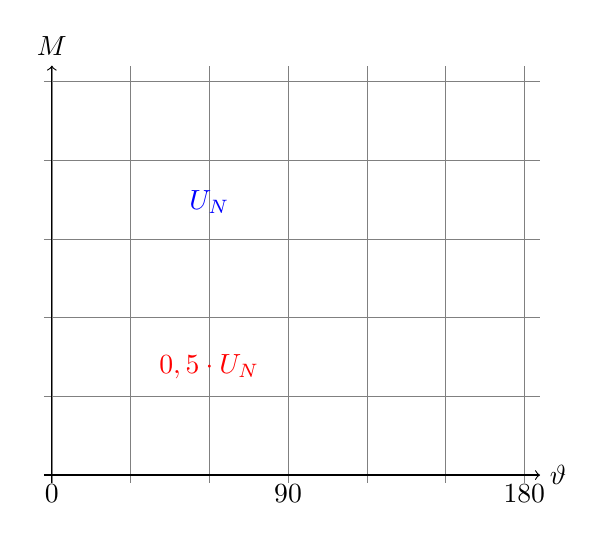
\begin{tikzpicture}[domain=0:6, samples=200]
	\draw[very thin,color=gray] (-0.1,-0.1) grid (6.2,5.2);
	\draw[->] (-0.1,0) -- (6.2,0) node[right] {$\vartheta$};
	\draw[->] (0,-0.1) -- (0,5.2) node[above] {$M$};
	\draw[color=red, smooth] plot[id=drehmomentkennlinie1] function{-x*x / 4 + 1.5 * x};
	\draw[color=red] (2,1.1) node[above] {$0,5\cdot U_N$};
	\draw[color=blue, smooth] plot[id=drehmomentkennlinie2] function{-x*x / 2 + 3 * x };
	\draw[color=blue] (2,3.2) node[above] {$U_N$};
	\draw (0,0) node[below] {0\degree};
	\draw (3,0) node[below] {90\degree};
	\draw (6,0) node[below] {180\degree};
\end{tikzpicture}